\chapter{Аналитическая часть}

В данном разделе будут описаны основные теоретические аспекты, необходимые для решения поставленной задачи.

\section{Протокол HTTP}

\textbf{HTTP} (англ. Hypertext Transfer Protocol, гипертекстовый транспортный протокол) \cite{http} --- протокол, определяющий набор соглашений по передаче гипертекста (т.е. связанных веб-документов) между двумя компьютерами. HTTP является текстовым протоколом без сохранения состояния.

Данный протокол задаёт следующие правила взаимодействия клиента и сервера. \cite{web_server}

\begin{itemize}[label*=---]
	\item HTTP-запросы производятся исключительно от клиентов к серверу, который способен только отвечать на запросы.
	\item При запросе файла по HTTP клиент должен сформировать файловый \textbf{URL} (Uniform Resource Locator, единообразный указатель местонахождения ресурса). \cite{url}
	\item Веб-сервер должен ответить на каждый HTTP-запрос, даже в случае возникновения ошибки.
\end{itemize}

HTTP-запросы и ответы имеют схожую структуру и состоят из следующих элементов. \cite{http_messages}

\begin{itemize}[label*=---]
	\item Начальная строка, описывающая запросы.
	\item Необязательный набор заголовков HTTP, определяющий запрос или описывающий тело сообщения.
	\item Необязательное тело сообщения, содержащее данные, связанные с запросом (например, содержимое HTML-формы), или документ, связанный с ответом. Наличие тела и его размер задаются начальной строкой и заголовками HTTP.
\end{itemize}

Начальная строка и HTTP-заголовки HTTP-сообщения вместе называются \textbf{заголовком}, а его полезная нагрузка --- \textbf{телом}. На рисунке \ref{fig:http} представлено описание структуры запроса и ответа HTTP версии 1.x. \cite{http_messages}

\begin{figure}[H]
	\centering
	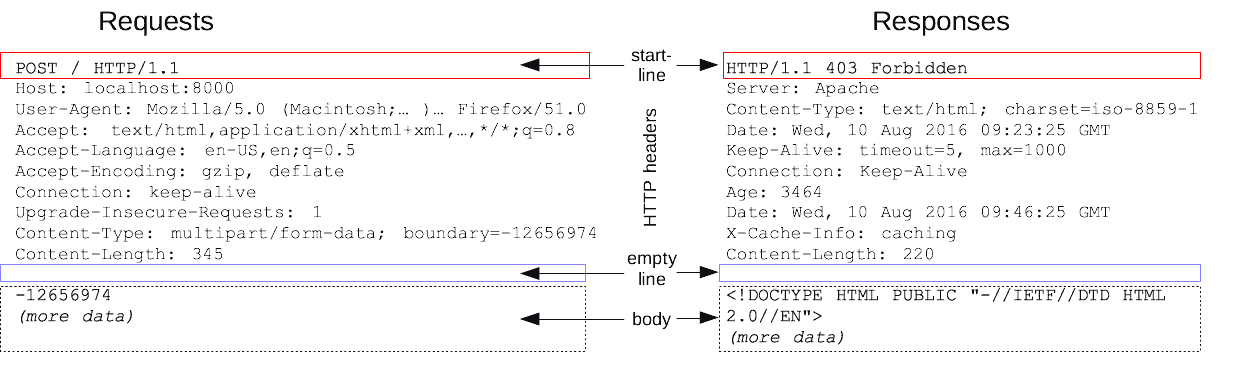
\includegraphics[width=\textwidth]{assets/http.png}
	\caption{Структура запроса и ответа HTTP версии 1.x}
	\label{fig:http}
\end{figure}



\section{Веб-серверы}

Веб-серверы, как правило, работают по протоколам HTTP/HTTPS и предоставляют клиентам доступ к файлам, таким как веб-страницы. Чтобы загрузить веб-страницу, браузер отправляет запрос к веб-серверу, который выполняет поиск запрашиваемого файла в своём хранилище. Найдя файл, сервер считывает его, обрабатывает при необходимости и отсылает в браузер. \cite{web_server}

Преимущества выделенных веб-серверов по сравнению с локальными хранилищами: \cite{web_server}

\begin{enumerate}[label*=\arabic*)]
	\item бесперебойная работа;
	\item постоянное подключение к интернету;
	\item неизменный IP адрес;
	\item обслуживание сторонним провайдером.
\end{enumerate}

Веб-серверы могут работать со статическим и динамическим контентом: статический отдаётся клиенту в исходном виде без изменений, а динамический является результатом обработки данных на стороне сервера. Со статическим контентом проще работать, в то время, как динамический контент обеспечивает большую гибкость. \cite{web_server}

\section{Сокеты}

\textbf{Сокет} --- это абстракция конечной точки соединения, которая используется для обеспечения обмена данными между устройствами сети. Сокеты являются ключевым компонентом для установки и управления сетевыми соединениями.

Сокеты предоставляют интерфейс для создания конечных точек соединения в сети с использованием протоколов передачи данных, таких как TCP или UDP. При разработке веб-серверов сокеты используются для <<прослушивания>> входящих соединений от клиентов и передачи данных между сервером и клиентами.

Процесс создания сервера с использованием сокетов включает в себя следующие шаги.

\begin{enumerate}[label*=\arabic*.]
	\item Создание сокета, который будет слушать входящие соединения.
	\item Привязка сокета к адресу и порту: после создания сокета необходимо привязать его к сетевому адресу и порту, на котором будет прослушиваться входящий трафик.
	\item Установка сервера в состояние прослушивания входящих соединений.
	\item Принятие входящего соединения.
	\item Обработка запросов и передача данных: После установки соединения с клиентом сервер может принимать запросы от клиента с помощью функций чтения и записи данных через сокет.
\end{enumerate}

Использование сокетов в разработке серверов позволяет эффективно управлять сетевыми соединениями и обеспечивать передачу статического контента клиентам по сети.



\section{Мультиплексирование ввода-вывода}

\textbf{Мультиплексирование} ввода-вывода является методом обработки нескольких операций ввода-вывода в одном потоке выполнения программы, что позволяет повысить эффективность управления множеством соединений в сетевых приложениях или приложениях с асинхронным вводом-выводом. Это позволяет уменьшить задержки и повысить производительность.

\textbf{Мультиплексоры} позволяют приложению ожидать ввода или вывода данных из нескольких источников, таких как сокеты, файлы или сетевые устройства, используя один системный вызов вместо создания или управления каждым потоком или процессом отдельно.

Использование мультиплексирования ввода-вывода требует более сложной логики обработки событий, чем простое параллельное программирование, но оно может обеспечить более эффективное использование системных ресурсов и более высокую производительность.

Существуют следующие механизмы мультиплексирования сетевых соединений.

\begin{itemize}[label*=---]
	\item \textbf{select} --- это системный вызов, используемый в различных операционных системах для ожидания событий на нескольких файловых дескрипторах, таких как сокеты. Он позволяет одному потоку контролировать несколько соединений одновременно. Данный мультиплексор имеет ограничение на максимальное количество отслеживаемых файловых дескрипторов --- 1024.
	\item \textbf{pselect} схож по принципу работы с select и имеет те же ограничения, однако реализует более продвинутую обработку сигналов.
	\item \textbf{epoll}, предоставляемый в ядре Linux, обеспечивает более гибкие варианты работы с событиями ввода-вывода за счёт реализации модели уведомлений. В отличие от select и pselect, epoll предоставляет более эффективный способ мониторинга множества файловых дескрипторов на предмет готовности к вводу или выводу и не имеет ограничений на обработку файловых дескрипторов.
\end{itemize}

epoll является наиболее современным и эффективным механизмом в сравнении с select и pselect и часто используется в высоконагруженных сетевых приложениях на ОС Linux.



\section{Параллелизация обработки запросов}

Для ускорения обработки запросов веб-серверы реализуют их параллельную обработку в многопроцессорной среде. Существует два подхода к параллелизации работы веб-серверов: пул потоков (thread pool) и разветвление (prefork).

\textbf{Thread Pool} представляет собой набор потоков, готовых к выполнению задач. Когда в систему поступает новая задача, она помещается в очередь, и один из доступных потоков в пуле забирает эту задачу на выполнение. После завершения задачи поток возвращается обратно в пул и становится доступным для выполнения новых задач. Это способствует уменьшению накладных расходов на создание и уничтожение потоков, а также позволяет управлять ресурсами более эффективно и обеспечивает параллельное выполнение задач.

\textbf{Prefork} --- это модель параллелизации, при которой веб-сервер создаёт отдельные процессы для обработки запросов. Такой подход позволяет изолировать обработку каждого запроса и повышает надежность веб-сервера, так как сбои в одном процессе не влияют на остальные. Однако создание процессов требует больше дополнительных ресурсов, чем использование пула потоков.

Выбор между Thread Pool и Prefork зависит от конкретных требований веб-сервера, предполагаемой нагрузки и характера обрабатываемых запросов.
